\documentclass{article}
\usepackage[english]{babel}
\usepackage[utf8]{inputenc}
\usepackage{amsmath,amssymb}
\usepackage{parskip}
\usepackage{graphicx}
\usepackage{dsfont}
\usepackage{dsfont}
\usepackage{relsize}
\usepackage{array}
\newcommand{\bigsigma}{\makebox{\Huge\ensuremath{\sigma}}}
\newcommand{\bigpi}{\makebox{\Huge\ensuremath{\Pi}}}
\newcolumntype{C}[1]{>{\centering\let\newline\\\arraybackslash\hspace{0pt}}m{#1}}
\usepackage[top=2.5cm, left=3cm, right=3cm, bottom=4.0cm]{geometry}
\usepackage[table]{xcolor}
\usepackage[utf8]{inputenc}
\usepackage{textcomp}
\usepackage[utf8]{inputenc}
\usepackage{amsmath}
\usepackage{amssymb}
\usepackage{xcolor}
\usepackage{listings}
\usepackage{xstring}
\usepackage{graphicx}
\usepackage[export]{adjustbox}
\usepackage{setspace}

\definecolor{dkgreen}{rgb}{0,0.6,0}
\definecolor{ltgray}{rgb}{0.5,0.5,0.5}

\makeatletter
\newif\ifcolname
\colnamefalse

\def\keywordcheck{%
\IfStrEq*{\the\lst@token}{select}{\global\colnametrue}{}%
\IfStrEq*{\the\lst@token}{where}{\global\colnametrue}{}%
\IfStrEq*{\the\lst@token}{from}{\global\colnamefalse}{}%
\color{blue}%
}
\def\setidcolor{%
\ifcolname\color{purple}\else\color{black}\fi%
}
\makeatother

\lstset{%
    backgroundcolor=\color{white},
    basicstyle=\footnotesize,
    breakatwhitespace=false,
    breaklines=true,
    captionpos=b,
    commentstyle=\color{dkgreen},
    deletekeywords={...},
    escapeinside={\%*}{*)},
    extendedchars=true,
    frame=single,
    keepspaces=true,
    language=SQL,
    otherkeywords={is},
    morekeywords={*,modify,MODIFY,...},
    keywordstyle=\keywordcheck,
    identifierstyle=\setidcolor,
    numbers=left,
    numbersep=15pt,
    numberstyle=\tiny,
    rulecolor=\color{ltgray},
    showspaces=false,
    showstringspaces=false, 
    showtabs=false,
    stepnumber=1,
    tabsize=4,
    title=\lstname
}
\makeatletter
\usepackage{color}
\definecolor{lightgray}{rgb}{0.95, 0.95, 0.95}
\definecolor{darkgray}{rgb}{0.4, 0.4, 0.4}
%\definecolor{purple}{rgb}{0.65, 0.12, 0.82}
\definecolor{editorGray}{rgb}{0.95, 0.95, 0.95}
\definecolor{editorOcher}{rgb}{1, 0.5, 0} % #FF7F00 -> rgb(239, 169, 0)
\definecolor{editorGreen}{rgb}{0, 0.5, 0} % #007C00 -> rgb(0, 124, 0)
\definecolor{orange}{rgb}{1,0.45,0.13}		
\definecolor{olive}{rgb}{0.17,0.59,0.20}
\definecolor{brown}{rgb}{0.69,0.31,0.31}
\definecolor{purple}{rgb}{0.38,0.18,0.81}
\definecolor{lightblue}{rgb}{0.1,0.57,0.7}
\definecolor{lightred}{rgb}{1,0.4,0.5}
\usepackage{upquote}
\usepackage{listings}
% CSS
\lstdefinelanguage{CSS}{
  keywords={color,background-image:,margin,padding,font,weight,display,position,top,left,right,bottom,list,style,border,size,white,space,min,width, transition:, transform:, transition-property, transition-duration, transition-timing-function},	
  sensitive=true,
  morecomment=[l]{//},
  morecomment=[s]{/*}{*/},
  morestring=[b]',
  morestring=[b]",
  alsoletter={:},
  alsodigit={-}
}

% JavaScript
\lstdefinelanguage{JavaScript}{
  morekeywords={typeof, new, true, false, catch, function, return, null, catch, switch, var, if, in, while, do, else, case, break},
  morecomment=[s]{/*}{*/},
  morecomment=[l]//,
  morestring=[b]",
  morestring=[b]'
}

\lstdefinelanguage{HTML5}{
  language=html,
  sensitive=true,	
  alsoletter={<>=-},	
  morecomment=[s]{<!-}{-->},
  tag=[s],
  otherkeywords={
  % General
  >,
  % Standard tags
	<!DOCTYPE,
  </html, <html, <head, <title, </title, <style, </style, <link, </head, <meta, />,
	% body
	</body, <body,
	% Divs
	</div, <div, </div>, 
	% Paragraphs
	</p, <p, </p>,
	% scripts
	</script, <script,
  % More tags...
  <canvas, /canvas>, <svg, <rect, <animateTransform, </rect>, </svg>, <video, <source, <iframe, </iframe>, </video>, <image, </image>, <header, </header, <article, </article
  },
  ndkeywords={
  % General
  =,
  % HTML attributes
  charset=, src=, id=, width=, height=, style=, type=, rel=, href=,
  % SVG attributes
  fill=, attributeName=, begin=, dur=, from=, to=, poster=, controls=, x=, y=, repeatCount=, xlink:href=,
  % properties
  margin:, padding:, background-image:, border:, top:, left:, position:, width:, height:, margin-top:, margin-bottom:, font-size:, line-height:,
	% CSS3 properties
  transform:, -moz-transform:, -webkit-transform:,
  animation:, -webkit-animation:,
  transition:,  transition-duration:, transition-property:, transition-timing-function:,
  }
}

\lstdefinestyle{htmlcssjs} {%
  % General design
%  backgroundcolor=\color{editorGray},
  basicstyle={\footnotesize\ttfamily},   
  frame=b,
  % line-numbers
  xleftmargin={0.75cm},
  numbers=left,
  stepnumber=1,
  firstnumber=1,
  numberfirstline=true,	
  % Code design
  identifierstyle=\color{black},
  keywordstyle=\color{blue}\bfseries,
  ndkeywordstyle=\color{editorGreen}\bfseries,
  stringstyle=\color{editorOcher}\ttfamily,
  commentstyle=\color{brown}\ttfamily,
  % Code
  language=HTML5,
  alsolanguage=JavaScript,
  alsodigit={.:;},	
  tabsize=2,
  showtabs=false,
  showspaces=false,
  showstringspaces=false,
  extendedchars=true,
  breaklines=true,
  % German umlauts
  literate=%
  {Ö}{{\"O}}1
  {Ä}{{\"A}}1
  {Ü}{{\"U}}1
  {ß}{{\ss}}1
  {ü}{{\"u}}1
  {ä}{{\"a}}1
  {ö}{{\"o}}1
}
%
\lstdefinestyle{py} {%
language=python,
literate=%
*{0}{{{\color{lightred}0}}}1
{1}{{{\color{lightred}1}}}1
{2}{{{\color{lightred}2}}}1
{3}{{{\color{lightred}3}}}1
{4}{{{\color{lightred}4}}}1
{5}{{{\color{lightred}5}}}1
{6}{{{\color{lightred}6}}}1
{7}{{{\color{lightred}7}}}1
{8}{{{\color{lightred}8}}}1
{9}{{{\color{lightred}9}}}1,
basicstyle=\footnotesize\ttfamily, % Standardschrift
numbers=left,               % Ort der Zeilennummern
%numberstyle=\tiny,          % Stil der Zeilennummern
%stepnumber=2,               % Abstand zwischen den Zeilennummern
numbersep=5pt,              % Abstand der Nummern zum Text
tabsize=4,                  % Groesse von Tabs
extendedchars=true,         %
breaklines=true,            % Zeilen werden Umgebrochen
keywordstyle=\color{blue}\bfseries,
frame=b,
commentstyle=\color{brown}\itshape,
stringstyle=\color{editorOcher}\ttfamily, % Farbe der String
showspaces=false,           % Leerzeichen anzeigen ?
showtabs=false,             % Tabs anzeigen ?
xleftmargin=17pt,
framexleftmargin=17pt,
framexrightmargin=5pt,
framexbottommargin=4pt,
%backgroundcolor=\color{lightgray},
showstringspaces=false,      % Leerzeichen in Strings anzeigen ?
}%
%


\makeatother


\newcommand{\tablespace}{\\[1.25mm]}
\newcommand\Tstrut{\rule{0pt}{2.6ex}}         % = `top' strut
\newcommand\tstrut{\rule{0pt}{2.0ex}}         % = `top' strut
\newcommand\Bstrut{\rule[-0.9ex]{0pt}{0pt}}   % = `bottom' strut
\title{Assignment-3 CS303}
\author{Shashank P \\ 200010048}
\date{\today}

\begin{document}
\maketitle




\section{Problem 1}
Design a database for an automobile company to provide to its dealers to assist them in maintaining
customer records and dealer inventory and to assist sales staff in ordering cars.
Each vehicle is identified by a vehicle identification number ( VIN ). Each individual vehicle is a
particular model of a particular brand offered by the company (e.g., the XF is a model of the car brand
Jaguar of Tata Motors). Each model can be offered with a variety of options, but an individual car may
have only some (or none) of the available options. The database needs to store information about models,
brands, and options, as well as information about individual dealers, customers, and cars. Your design
should include an E-R diagram, a set of relational schemas, and a list of constraints, including
primary-key and foreign-key constraints.


\begin{figure}[!ht]
  \begin{center}
    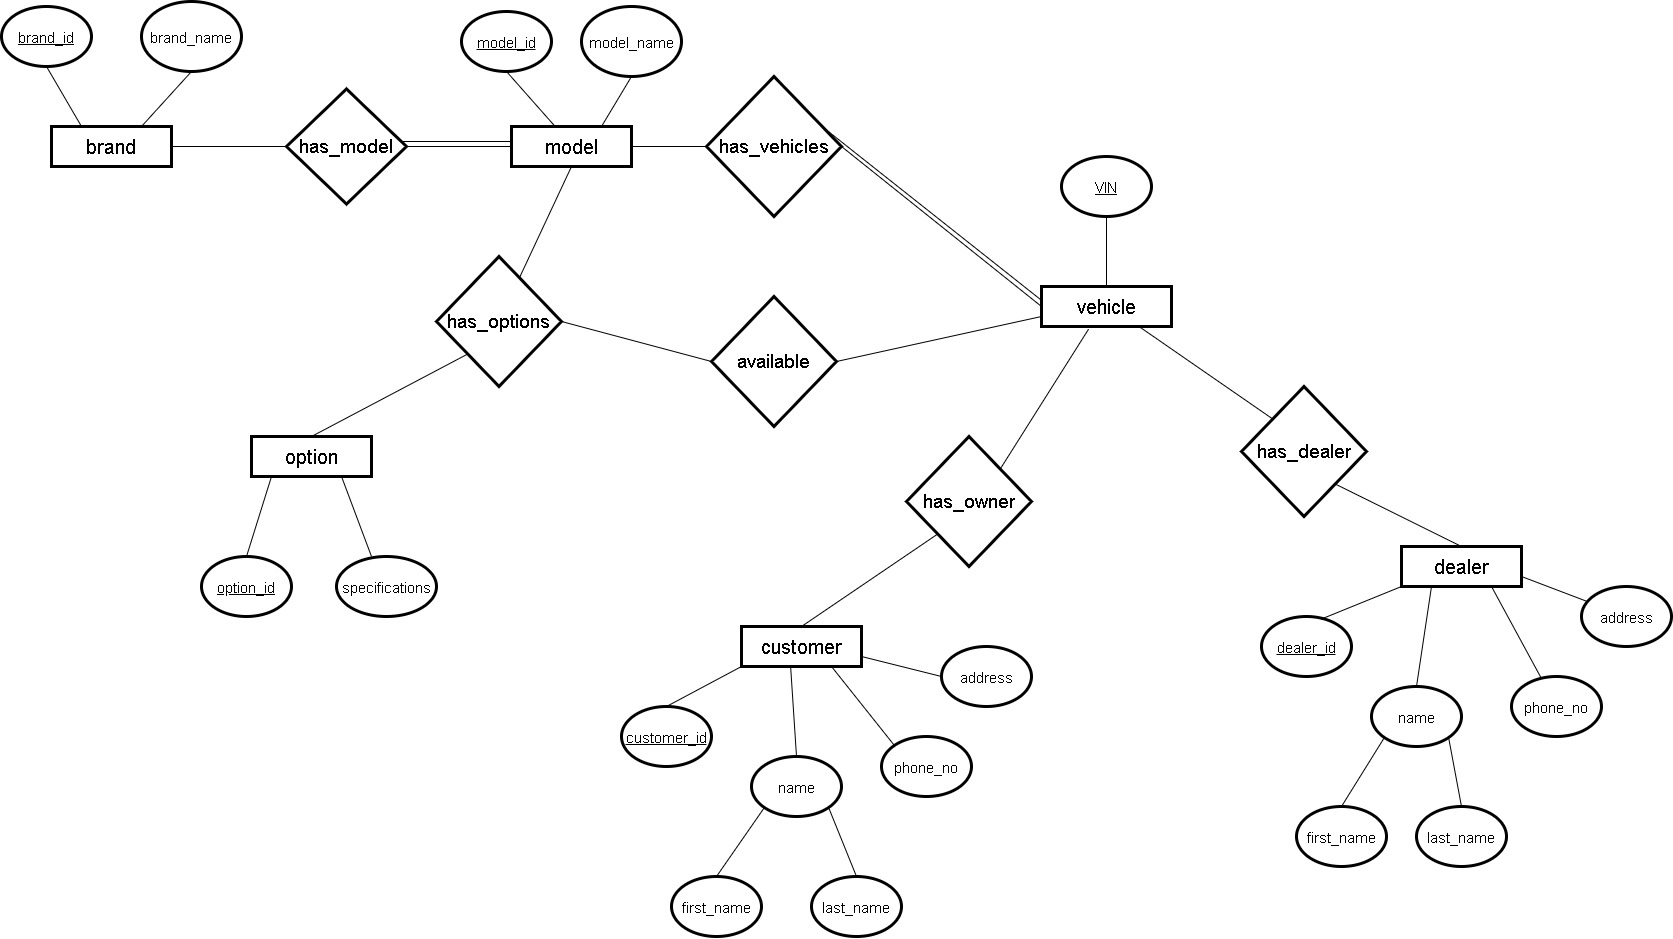
\includegraphics[scale=0.3]{1.jpg}
  \caption{ER Model}
  \end{center}
\end{figure}

\subsection{Schema}
\onehalfspacing
\begin{center}
  brand (\underline{brand\_id}, brand\_name), \\
  model (\underline{model\_id}, mdoel\_name), \\
  option (\underline{option\_id}, specifications), \\
  vehicle (\underline{VIN}), \\
  customer (\underline{customer\_id}, name, phone\_no, address), \\
  dealer (\underline{dealer\_id}, name, phone\_no, address), \\
  has\_model (\underline{brand\_id} ref. \textbf{brand}, \underline{model\_id} ref. \textbf{model}), \\
  has\_options (\underline{model\_id} ref. \textbf{model}, \underline{option\_id} ref. \textbf{option}), \\
  has\_vehicles (\underline{model\_id} ref. \textbf{model}, \underline{VIN} ref. \textbf{vehicle}), \\
  available ((\underline{model\_id}, \underline{option\_id}) ref. \textbf{has\_options}, \underline{VIN} ref. \textbf{vehicle}), \\
  has\_owner (\underline{VIN} ref. \textbf{vehicle}, \underline{customer\_id} ref. \textbf{customer}), \\
  has\_dealer (\underline{VIN} ref. \textbf{vehicle}, \underline{dealer\_id} ref. \textbf{dealer}) \\
\end{center}

\section{Problem 2}
Design a database for a world-wide package delivery company (e.g., DHL or Fed EX ). The database
must be able to keep track of customers (who ship items) and customers (who receive items); some
customers may do both. Each package must be identifiable and trackable, so the database must be able to
store the location of the package and its history of locations.
Locations include trucks, planes, airports, and warehouses. Your design should include an E-R diagram, a
set of relational schemas, and a list of constraints, including primary-key and foreign-key constraints.

\newpage
\begin{figure}[!ht]
  \begin{center}
    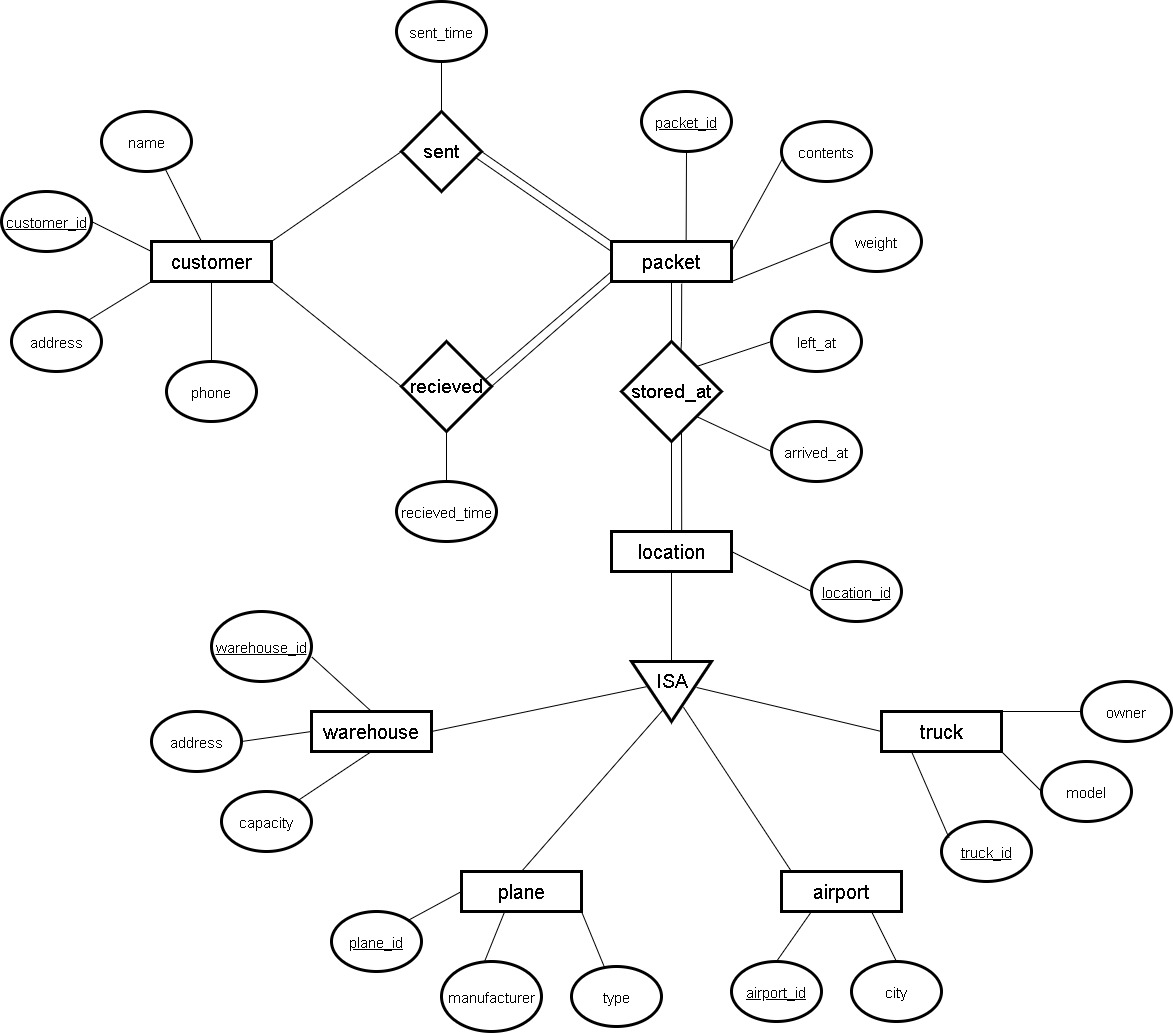
\includegraphics[scale=0.4]{2.jpg}
  \caption{ER Model}
  \end{center}
\end{figure}

\newpage
\subsection{Schema}
\onehalfspacing
\begin{center}
  customer (\underline{customer\_id}, name, phone, address), \\
  packet (\underline{packet\_id}, contacts, weight), \\
  location (\underline{location\_id}), \\
  warehouse (\underline{warehouse\_id} ref. \textbf{location(location\_id)}, address, capacity), \\
  plane (\underline{plane\_id} ref. \textbf{location(location\_id)}, manufacturer, type), \\
  airport (\underline{airport\_id} ref. \textbf{location(location\_id)}, city), \\
  truck (\underline{truck\_id} ref. \textbf{location(location\_id)}, model, owner), \\
  sent (\underline{customer\_id} ref. \textbf{customer}, \underline{packet\_id} ref. \textbf{packet}, sent\_time), \\
  recived (\underline{customer\_id} ref. \textbf{customer}, \underline{packet\_id} ref. \textbf{packet}, recieved\_time), \\
  stored\_at (\underline{packet\_id} ref. \textbf{packet}, \underline{location\_id} ref. \textbf{location}, arrived\_at, left\_at), \\
\end{center}


\section{Problem 3}
Since the HTML page will be publicly available to everyone as it is client-side, a user can edit the HTML page's source code to replace the old price value with the new one. The server would not know whether the user modified the price value and would place the order using the modified price.

\section{Problem 4}
Even though a link is visible only to an authorized user, an unauthorized user may somehow know of the URL's existence (for example, via Web history logs). The user may then log in to the system and access the unauthorized page by entering its URL in the browser. If the check for user authorization were left out from that page, the user would be able to see the result of the page. The HTTP referer attribute can be used to block such loopholes by ensuring the referer value is from a valid page of the Web site. However, the browser sets the referrer attribute, so a malicious user can quickly work around the referer check.

\section{Problem 5}
HTTPS protocol is used to prevent multiple types of attacks, by ensuring that
the HTTP request being sent is encrypted using public / private key encyption
and also whether the request is going to the intended user using digital certificates.

\begin{enumerate}
  \item HTTPS encrypts the request sent from the end user, which can only be decrypted by 
        server. This prevents hackers from viewing or modifying the request on route.
  \item Buying an SSL certificate from a verified company, allows the company to sign the public key.
        This SSL certificate can be used by the website to show users that it is actually the website that they are trying to access and not a malicious one.
        
  \item If the website has an SSL certificate it will have \textbf{https} pad-lock.

\end{enumerate}

\section{Problem 6}
The login HTML is shown below.
\begin{lstlisting}[style=htmlcssjs]
<!DOCTYPE html>
<html>
  <head>
    <title>Login</title>
  </head>
<body>
  <form action="LoginServlet" method="post">
    User ID: <input type="text" name="userid"> <br>
    Password: <input type="password" name="password"> <br>
    <input type="submit" value="Login">
  </form>
</body>
</html>
\end{lstlisting}

The LoginServlet used to handle login, is shown below.
\begin{lstlisting}[language=java]
  @WebServlet("/LoginServlet")
  public class LoginServlet extends HttpServlet {
    private static final long serialVersionUID = 1L;
  
    protected void doPost(HttpServletRequest request,
        HttpServletResponse response) throws ServletException, IOException {
      try{
        // Getting the request parameters
        String userid = request.getParameter("userid");
        String password = request.getParameter("password");
        
        // Connecting to mysql databse
        Connection con = null;
        String url = "jdbc:mysql://localhost:3306/users"; //MySQL URL and followed by the database name
        String username = "root"; //MySQL username
        String password = "password"; //MySQL password
        Class.forName("com.mysql.jdbc.Driver");
        con = DriverManager.getConnection(url, username, password);

        // Create Prepaared Statement
        PreparedStatement check = con .prepareStatement("select userid, password from data where userid=? and password=?");
 		    check.setString(1, userid);
 		    check.setString(2, password);

        // Execute the query
        ResultSet rs = check.executeQuery();
        
        // Check output of query
        if(rs.isBeforeFirst()){
          while(rs.next()){
            // Creating a session cookie
            Cookie loginCookie = new Cookie("userid", rs.getString("userid"));

            // Setting cookie to expiry
            loginCookie.setMaxAge(30*60);

            // Adding the cookie to the response
            response.addCookie(loginCookie);
            response.sendRedirect("LoginSuccess.jsp");
          }
        }else{

          // Login Error if user or password do not match 
          RequestDispatcher rd = request.getRequestDispatcher("LoginError.jsp");
          rd.forward(request, response);
        }
      }catch(Exception e) {

        // General Exception Handling.
        e.printStackTrace();
        RequestDispatcher rd = request.getRequestDispatcher("Error.jsp");
        rd.forward(request, response);
      }
  
    }
  
  }
\end{lstlisting}

This will set a session cookie named \textbf{userid} after the user logs in successfully, but gives an error
in all other cases.

\section{Problem 7}
XSS or Cross-Site Scripting is a client side code injection attack. In this
type of attack, the malicious user tries to inject code into legitimate websites.
These websites then become a carrier of malicious code, which effects other users
who use the website. \\

Most common place of injections include message boards, forums, discussion websites, text input output based services.
The attack can occur if the server does not filter the request for malicious code and tries to render the text 
given as input without checking for hidden code. \\

Ways of preventing an XSS attack are
\begin{enumerate}
  \item Secuirty training and awareness needs do be given to the developers, ops team, etc., before they start building an application.
  \item Do not trust any input that comes from the user, requests needs to go through a trusted filtering process.
  \item Using text formatters such as prepareStatement, string formatter, etc., to execute user inputs.
  \item Parse and clean the HTML page to be returned using trusted libraries.
  \item Use HttpOnly cookies which prevent client side users from modifying cookies.
  \item Content Security Policy allows you to declare where and how a dynamic code snippet can be executed.
\end{enumerate}


\end{document}
